\addbibresource{reference.bib}

\chapter{Úvod do hybridních částicových pixelových detektorů}\label{chap:detectors}
Ionizující záření je lidskými smysli nedetekovatelné, avšak jeho studie nám umožňuje pochopit podstatu hmoty, její vlastnosti a interakce. To lidstvu umožnilo mnohé aplikace, jako je na příklad protonová terapie, defektoskopie nebo zkoumání pravosti uměleckých děl. První pokusy o detekci ionizujícího záření sahají do počátku 20. století, kde pomocí mlžné komory se prvně podařilo zachytit trajektorii nabitých částic. Rozvoj polovodičové technologie dal vzniku novým detekčním technologiím až po v současné době nejpokrokovějším - pixelovým detektorům.

Existuje celá řada částicových pixelových detektorů, ale v této kapitole budou popsány jen hybridní pixelové detektory, pro které je typické, že se skládají ze dvou nezávisle vyrobených částí - senzoru a vyčítacího čipu. To oproti monolitickým detektorů, kde vyčítací elektronika je součástí senzoru přináší řadu výhod, jako na příklad snížení výrobních nákladů nebo možnost kombinace vyčítacího čipu se senzory různých materiálů (\textit{Si}, \textit{GaAs}, \textit{CaTe} apod.).

Na tomto místě je třeba zmínit, že existuje více druhů těchto detektorů (\textit{AGH Fermilab, Pilatus, Philips Chromaix} apod.)[\cite{detectors_review}], v této práci budou použity použity pouze detektory z rodiny detektorů Medipix/Timepix.


\section{Hardwarová architektura}
\begin{figure}[th]
	\begin{center}
		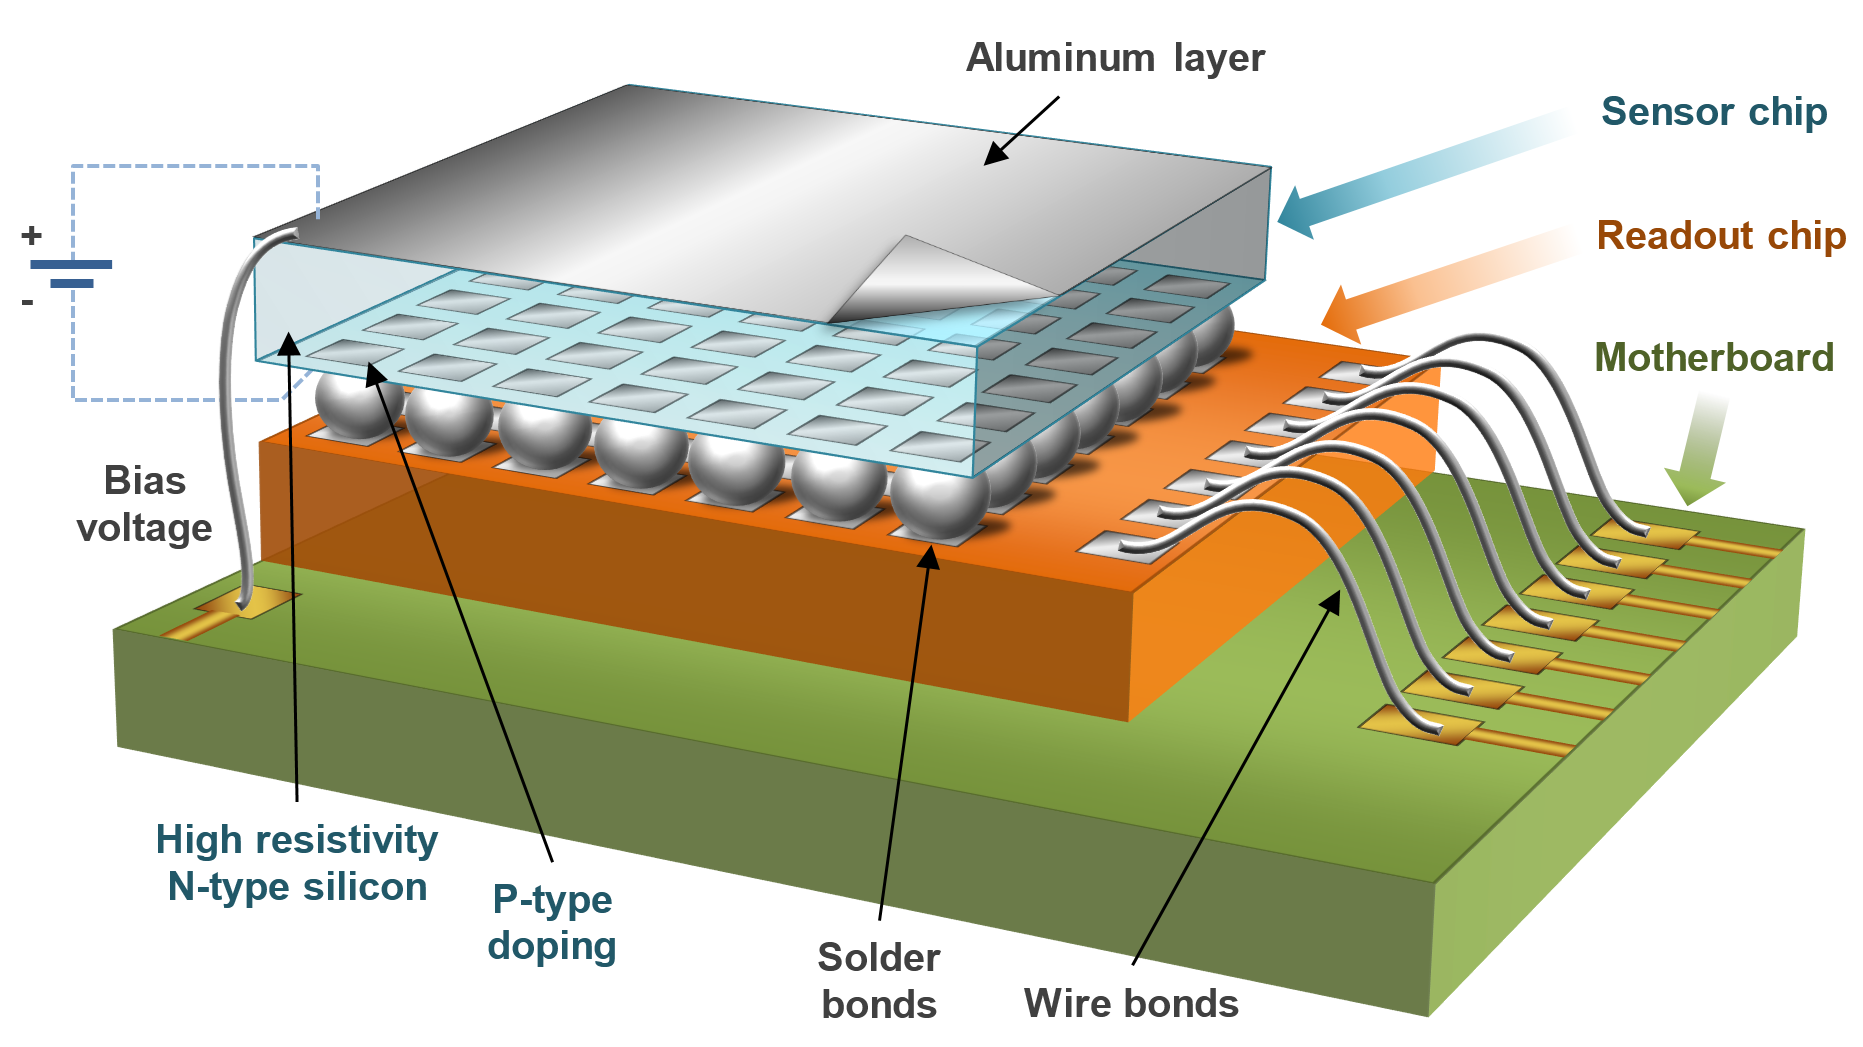
\includegraphics[width=12cm]{figures/det_chip.png}
		\caption{Struktura hybridního polovodičového pixelového detektoru Timepix3, skládající se z vyčítacího čipu a polovodičového senzoru (převzato z~\cite{PlatkevicDisertace}).}
		\label{fig:det:chip}
	\end{center}
\end{figure}
Většina hybridních částicových pixelových detektorů rodiny Medipix/Timepix obsahuje matici $256\times256$ pixelů. Každý z nich má stanu o délce $55~\mu m$, takže senzor čítající $65536$ má plochu $1.4 \times 1.4 cm^2$.